\documentclass[12pt]{article}
\usepackage{fancyhdr}
\usepackage{lastpage}\usepackage{amsmath,amssymb,amsfonts,mathrsfs,latexsym}
\usepackage{amsthm}
\usepackage{ulem}
\usepackage{graphicx}
\usepackage{enumerate}
\usepackage{enumitem}
\usepackage{float}
\usepackage{caption}
\usepackage{mathtools}
\usepackage[]{hyperref}
\usepackage[margin=2.5 cm,includehead,includefoot]{geometry} %Til at ændre marginen
\usepackage{framed,color}
\usepackage[explicit]{titlesec}
\usepackage{pstricks}
\usepackage{xcolor}
\usepackage{xparse}
\usepackage{caption}
\usepackage{multirow}
\usepackage{subcaption}
\usepackage[english]{babel}
\usepackage[utf8]{inputenc}
\setlength\parindent{0pt}
\usepackage[backend = bibtex]{biblatex}
\addbibresource{bibliography.bib}
%\bibliography{bibliography.bib}
%fjerner indryk ved linjeskift
%nye kommandoer til at lave symboler for talmængder
%Input til at udfylde forside og sidehoveder
\newcommand{\kuid}{KNJ284}
\newcommand{\flnavn}{Patrik H. Rauff}
\newcommand{\kfal}{P. H. Rauff}
\newcommand{\hold}{}
\newcommand{\deadline}{}
\newcommand{\fag}{xIBOR in transition}
\newcommand{\shortfag}{PUK , xIBOR in transition}
\newcommand{\ku}{University of Copenhagen}
\newcommand{\cphu}{University of Copenhagen}
\newcommand{\opg}{Project out of Cource Scope}
%forside
\author{\textbf{\textsl{\flnavn}} \ \textbf{\textsl{\kuid}} \ \textbf{\textsl{\hold}}}
\title{\fag \\ \ku \\ \opg }
\date{}
%Sidehoved og -fod
\pagestyle{fancy}
\chead{}
\lhead{\kfal, \kuid \\ \shortfag \pagebreak}
\rhead{\cphu \\ \date{\today}}
\lfoot{}
\cfoot{{Side \thepage \hspace{1pt} af \pageref{LastPage}}}
\rfoot{}
\begin{document}
\maketitle
\pagebreak
\tableofcontents
\pagebreak
\section{Introduction} % (fold)
After the 2007-2008 Global Financial Crisis
the era of single-curve term structure modelling
were jeopardized due to the
big spread occuring between the
OIS and xIBOR rates in the market
and thus the start of the era for multicurve modelling.
However the xIBOR rates plunged in popularity
and in 2012 the scandal of LIBOR manipulation
did not help for its reputation. The final
blow the the LIBOR rates where made in 2017,
where it was annouced that LIBOR was
to discountinue by the end of 2021. However the most important
Libor, the USD LIBOR is still live until 30 June 2023.
Although our focus will be on the EURO market (EURIBOR vs. €STR) -
even though EURIBOR has not yet (and maybe never will) be set to discontinue.\newline

This project is a proof of concepts on the
transition from the xIBOR rates to the OIS/RFR\footnote{The
terminology is a bit loose throughout the project. Whenever
OIS or RFR is mentioned it shall be understood
as the 'Risk-free' short term rates, which
is the reference rates for discounting.} rates
as the underlying floating rates for derivative contracts.
Although mostly traded, we will not consider the impact
of linearly interest rate derivatives, such as interest rate swaps,
since the transition should have a higher impact on
the non-linear derivatives such as Caplets and Caps.\linebreak

As another limitation of this project, we will
take on the challenge of the transition from forward-looking
to backward-looking rates such as covered in \cite{LyaMer2019FMM}
This is a whole theme on itself.

\section{The setup} % (fold)
\label{sec:the_setup}
We consider a probability space $(\Omega, \mathcal{F}, \left\{ \mathcal{F}_t \right\}_{0 \leq t \leq T^\star} , \mathbb{Q})$
Where we model the OIS rate as a classical short rate model ala Vasicek, hence:
\begin{equation}\label{eq:vasicekdynamics}
    dr(t) = \kappa \left[\theta - r(t) \right]dt + \sigma d W(t)
\end{equation}
where $W(t)$ is a
brownian motion under the risk-neutral $\mathbb{Q}$-measure.
The OIS rate also is the bedrock for our discounting factor,
which thus make our pricing consistent with
standard CSA pricing of derivative contracts, ie:
\begin{equation}
    P_D(t,T) = \mathbb{E}^\mathbb{Q}_t \left\{ e ^{- \int_{t}^{T}r_s ds} \right\}
\end{equation}
The convenient thing with the short rate above
is firstly that it is Gaussian and thus explicit computation
on bond prices are possible.
Given an initial short rate, $r(t)$,
the price of a Zero-Coupon Bond
 in the Vasicek model is
commonly known as:
\begin{equation}\label{eq:VasicekZCB}
    \notag P(t,T ; r(t)) = e ^{A(t,T) - B(t,T) r(t)}
\end{equation}
where
\begin{equation}\label{eq:AffineVasicek}
    \begin{aligned}
       & B(t,T) = \frac{1 - e ^{-\kappa(T-t)}}{\kappa} \\
       & A(t,T) = \left[\theta -
       \frac{\sigma^2}{\kappa^2}\right]
       \left\{ B(t,T) - (T-t) \right\}
       - \frac{\sigma^2}{4\kappa}B^2(t,T)
    \end{aligned}
\end{equation}
We consider derivative contracts starting at some time $T_0$
and has paying dates at $T_1<\dots < T_N$, where
$\tau ^x_k = T_k - T _{k-1}$ is the year fraction between two payment dates
and $x$ is the tenor-structure of the contract.
We will consider the most common tenor structures
namely $x = \left\{ 3\text{M} , 6\text{M}  , 12\text{M} \right\}$
and keep the time between payments fixed, whenever a tenor structure has been
chosen for a given contract ie. $\tau^{3\text{M}}_k = \tau ^{3\text{M}}$
for $k = 1,\dots,N$.
Another important building block
upon pricing OIS intstruments, and finding
the relation between the OIS and xIBOR rates are
made through the simply-compounded forward
rates given by:
\begin{equation}
    F_k^x (t) = \frac{1}{\tau_k^x} \left\{ \frac{P_D(t,T_{k-1})}{P_D(t,T_k)}-1 \right\}
\end{equation}

Along the lines of \cite{MercXieStochBasis2012} we consider the
a model where the OIS-xIBOR spread is addative, ie:
\begin{equation}
    \mathcal{S}_k^x(t) = L_k^x(t) - F_k^x(t)
\end{equation}
and is modelled by:
\begin{equation}\label{eq:BasisSpreadDef}
     S_k^x(t) = S_k^x(0) +
    \alpha_k^x \left[L_k^x(t) - L_k^x(0)\right] +
    \beta^x_k \left[\mathcal{X}_k^x(t) - \mathcal{X}_k^x(0)\right],\quad \mathcal{X}_k^x(0)=1
\end{equation}
Here $\mathcal{X}_k^x(t)$ is the stochastic basis factor,
which can be modelled in different ways. However we are
only interested in modelling $\mathcal{X}_k^x(t)$ in a
way that leads to simple and explicit computations of
xIBOR contracts. Initially we model the stochastic basis as a
martingale brownian motion :
\begin{equation} \label{eq:StocBasis}
     d\mathcal{X}_k^x(t) = \eta ^x _k(t) \mathcal{X}_k^x(t) dB_k^x(t)
\end{equation}
with $dB_k^x(t)$ is a Brownian motion independent of the $\mathbb{Q}$- and
$T^k_D$ forward measure.
\section{Pricing in the different models:}
\subsection{The OIS model}
\textbf{Pricing Caplets:}
under $\mathbb{Q}$ for $t \leq T_{k-1}$ we have:
\begin{equation}
    \notag Cpl(T _{k-1} , T_k , K , N; t) =
    \mathbb{E}^\mathbb{Q}_t
    \left\{ e ^{-\int_t ^{T_k} r_s ds}
    N\left[F_k^x(t) - K\right]^+\right\}
\end{equation}
With some change-of-measure trickery we are able to
price the Caplet in a Black like formula as in \cite{IRModels}:
\begin{equation}
    Cpl^{\text{OIS}}(T_{k-1},T_k , K ; t) =
    \left[P_D(t,T_{k-1}) \Phi(-d + \tilde \sigma_k)
    - (1+\tau_k^x K) P_D(t,T_k) \Phi(-d)\right]
\end{equation}
where $\Phi$ is the CDF for the Gaussian distribution
and
\begin{equation}
    \notag \tilde \sigma_k = \sigma \sqrt{\frac{1-e ^{-2\kappa(T_{k-1} - t)}}{2\kappa}}
    B(T_{k-1} , T_k),\quad
     d = \frac{1}{\tilde \sigma_k}\log
     \left\{ \frac{(1+\tau_k^x K )P_D(t,T_k)}{P_D(t,T_{k-1})} \right\}
     + \frac{\tilde \sigma _k}{2}
\end{equation}
And since a Cap of a given payment structure
$\mathcal{T}= \left\{ T_1 , \dots , T_n \right\}$ with:
\begin{equation}
    Cap ^{\text{OIS}}(T_0 , \mathcal{T} , K , N ; t )
    = N \sum_{k=1}^n Cpl ^{\text{OIS}}
    (T_{k-1} , T_k , K , N ; t)
\end{equation}
\subsection{The Spread Model}
In the Spread model it is not
quite as trivial since we have two stochastic processes
to take into account.
Firstly we consider the discounted payoff of a Cap at a
fixing date $T_{k-1}$ which pays at $T_k$:
\begin{equation}
    \notag \left[L_k^x(T_{k-1}) - K\right]^+  \tau_k^xP_D(T_{k-1},T_k)
\end{equation}
since our two stochastic parameters of $r(t)$ and $\mathcal{X}_k^x(t)$
are independent we can
without much endeavor find a semianalytical
solution, which only makes forces us to compute one integral
numerically. Recalling that a caplet is
just a one-period swaption with equal paying
structures for the fixed and floating leg, we
are lucky that it is just a simplified version
of the semi-analytical swaption pricing formula in
\cite{MercXieStochBasis2012}. Hence the
time 0 caplet price for a given
tenor structure\footnote{We
supress the tenor notation on the time parameters
to ease notation, since
it is embedded in the difference between the start
and maturity of the caplet.} computed as:
\begin{equation}
    \begin{aligned}
        Cpl^{\text{Spr}}
        (T_{k-1} , T_k , K;0) & =
        P_D(0,T_{k-1})\mathbb{E}^{T_k^x}_0 \left\{
        \left[L_k(T_{k-1}) - K\right]^+  \tau_k P_D(T_{k-1},T_k)
         \right\} \\
         & =
         \int_{-\infty}^{\infty} h \left\{ C(r) ,
         D(r) , V_\mathcal{X}(T_{k-1}) \right\}
         \frac{1}{\sqrt{2\pi \nu(T_{k-1})}}
         e ^{-\frac{\left(r-\mu
         \left( T_{k-1} \right) \right )^2}
         {2 \nu( T_{k-1})}}
         dr
    \end{aligned}
\end{equation}
Where:
\begin{equation}
    \begin{aligned}
        \mathbb{E}^{T}_t\left\{ r(T) \right\}
    &= \mu(T) = r(t)e ^{- \kappa(T- t)}
    + \left[\theta\kappa
    - \frac{\sigma ^2}{\kappa}\right]
    B \left( t, T \right)  +
   \frac{\sigma^2}{2} \left[
   e ^{-\kappa(T) - t} - e ^{-2\kappa (T- t)}\right] \\
   \mathbb{V}^T_t \left\{ r(T) \right\}
  & = \nu(T) = \frac{\sigma^2}{2\kappa} \left[
  1- e ^{-2 \kappa(T - t)} \right] \\
       \mathbb{V}_t ^T
        \left\{ \log(\mathcal{X}_(T_{k-1})) \right\} &
        = V_\mathcal{X}(T_{k-1}) = \sqrt{\int_{t}^{T_{k-1}} \eta(s)^2 ds}
    \end{aligned}
\end{equation}
and
\begin{equation}
    \begin{aligned}
        C(r) & \triangleq
        \tau_k P_D \left( T_{k-1} , T_k \right)
        \beta_k \\
        D(r) & \triangleq
        \left\{ \tau_k K + 1 + \alpha_k - \xi_k \tau_k \right\}
        P_D \left( T_{k-1},T_k \right)
        - (1+ \alpha_k) \\
        \xi_k &\triangleq
        L_k(0) - (1+\alpha_k)F_k(0) - \beta_k \\
        h(C,D,V) & \triangleq
        \begin{cases}
            \text{Bl}(C,D,V , 1), & \text{if }A,B > 0 \\
            \text{Bl}(-C,-D,V , -1), & \text{if }A,B < 0 \\
            C - D, & \text{if }A \geq 0, B \leq 0 \\
            0 , & \text{if }A \leq 0, B \geq 0
        \end{cases} \\
        \text{Bl}(F,K,v,\psi) & \triangleq
        \psi F \Phi \left[\psi\frac{\log \left( F/K \right)
        + v ^2 /2 }{v}\right]- \psi K \Phi
        \left[\frac{\log \left( F/K \right)
        - v ^2 /2 }{v}\right]
    \end{aligned}
\end{equation}
And as above we may price a Cap with payment structure
$\mathcal{T}$ and notional $N$:
\begin{equation}
    Cap ^{\text{Spr}}(T_0,\mathcal{T},K,N;0) =
    N \sum_{k=1}^n Cpl^{\text{Spr}}(T_{k-1},T_k , K ; 0)
\end{equation}
\section{Working with data}
It has been possible to fetch some market data on
the following EUR Data in the period 21.03.2022 to 17.03.2023:
The data is denoted as $i$ for a given date
and $TN$ for a point on the curve.:
\begin{itemize}
    \item €STR SWAP Curve - $SW_i^{TN}$
    \item EUR SWAP Curve with 3M EURIBOR a reference - $SW3M_i^{TN}$
    \item EUR Basis swap: €STR Swap vs. 3M EURIBOR -  $BS3M_i^{TN}$
    \item EUR Basis swap: 3M EURIBOR vs. 6M EURIBOR - $BS3M6M_i^{TN}$
\end{itemize}
Now the question at hand would be -
what to do with this market data? Well
Many things are possible, but we will merely use it for
finding the depencence structure for our spread model, ie.
determining $\alpha_k$ and $\beta_k$ in (\ref{eq:BasisSpreadDef}).
Furthermore we use the data initial curve
fitting for the forward xIBOR curve, which in our case
is the 3M and 6M EURIBOR.\footnote{If
one would have been smart enough, one could also have fitted the
initial €STR curve to a Hull-White model, so
the Risk-free rate model is realistic to market
data.}
\subsection{Determining $\alpha_k$ and $\beta_k$ from data:} % (fold)
\label{sub:determining_depedence}
To determine $\alpha_k$ and $\beta_k$
we find some inspiration from Section 3.1 in \cite{MercXieStochBasis2012},
since we set them to depend
on the correlation between basis swaps and the OIS Swap rate in
addition to the variance of basis swaps. Hence
for a given tenor structure $x$ we set:
\begin{equation}
     \alpha^x_k = \alpha^x = \rho ^{x} v^{x},
     \quad\beta_k^x = \beta^x = \frac{1}{2}\sqrt{1- ( \rho^{x})^2}v^x
\end{equation}
in \cite{MercXieStochBasis2012} they
set:
\begin{equation}
     \notag \rho_k ^x = \text{Corr}(S_k^x(T_{k-1}^x) , F_k(T_{k-1}^x)),
     \quad v^x_k = \sqrt{\mathbb{V}\left( S_k^x(T_{k-1}) \right) }
 \end{equation}
Since basis swaps are normally
quoted from 1 year and up to around 30 years,
we consider the correlation from year to year independent of each other.
In this way we break down the
correlation year by year between a Basis Swap curve and
one part of the corresponding Basis
swap(the €STR side of basis swap).
It is important to stress that this is not
quite as in \cite{MercXieStochBasis2012}, where they
model the correlation between the basis spread and
the OIS Forward rates:

Our method on the other hand measures the correlation between
the €STR swap rates and the corresponding
basis swap from €STR to a swap referencing
3M \& 6M EURIBOR respectively \newline

\textbf{Basis Spread for $x = $ 3M:}\newline
Here we set $S_k^{3M} = BS3M^{TN}$ the correlation and standard deviation
is thus:
\begin{equation}
    \notag \begin{aligned}
        \rho^{3M}_{TN} &= \text{Corr} \left(BS3M^{TN} , SW^{TN}  \right)
    \\ v^{3M}_{TN} & = \sqrt{\mathbb{V} \left( BS3M^{TN} \right)}
    \end{aligned}
\end{equation}
Table~\ref{tab:Corr3MBasis} leaves an overview of the historical
yearly correlations between the €STR vs. 3M Euribor Basis swap
and €STR swap rate:
\begin{table}[H]
    \centering
    \begin{tabular}{|c|c|c|c|}
    \hline
    & Min (at 1Y) & Max (at 25Y) & Avg. \\ \hline \hline
    $\rho^{3M}$ & -0.8098&   -0.3597& -0.60232 \\ \hline
    \end{tabular}
    \caption{Minimum, Maximum and average of the
    yearly correlations between the €STR swap rate
    and the €STR/3M EURIBOR basis swap}
    \label{tab:Corr3MBasis}
\end{table}
furthermore we compute the historical standard deviations,
were the summary is found in
Table~\ref{tab:Var3MBasis}.
\begin{table}[H]
    \centering
    \begin{tabular}{|c|c|c|c|}
    \hline
        & Min (at 30Y) & Max (at 1Y) & Avg.  \\ \hline \hline
      $v^{3M}$ & 0.0218 & 0.04491 & 0.03316  \\ \hline
    \end{tabular}
    \caption{Standard deviations for the €STR vs. 3M Euribor
    basis swap.}
    \label{tab:Var3MBasis}
\end{table}
\textbf{Basis Spread for $x = 6M$:}\newline
For this we unfortunately does not have
any directly observed basis spread, but we construct our
own through adding the 3M vs. 6M EURIBOR basis swap to
our €STR vs. 3M EURIBOR basis swap. Thus we define:
\begin{equation}
    \notag S^{6M}_k = S_k^{3M} + BS3M6M^{TN}
\end{equation}
A method that is practioned in the industry,
when directly basis swaps are not traded.
As above we thus have the correlation and standard deviation:
\begin{equation}
    \notag \begin{aligned}
        \rho^{6M}_{TN} &= \text{Corr} \left(BS3M^{TN} + BS3M6M^{tn} , SW^{TN}  \right)
    \\ v^{6M}_{TN} & = \sqrt{\mathbb{V} \left( BS3M^{TN} + BS3M6M^{TN} \right)}
    \end{aligned}
\end{equation}
At last we compute the historical yearly correlation and standard deviations
as above. And the summary for the historical estimates can be found
in Table~\ref{tab:Corr6MBasis} and Table~\ref{tab:stdDev6MBasis} respectively.
\begin{table}[H]
    \centering
    \begin{tabular}{|c|c|c|c|}
    \hline
        &Max (at 1Y) & Min (at 25Y) & Avg  \\ \hline \hline
       $\rho^{6M}$& -0.48192 & -0.66764 & -0.62067  \\ \hline
    \end{tabular}
    \caption{Historical correlations between our synthetic created €STR vs. 6M EURIBOR
    basis swap and €STR Swap rate}
    \label{tab:Corr6MBasis}
\end{table}
\begin{table}[H]
    \centering
    \begin{tabular}{|c|c|c|c|}
    \hline
            &  Min (at 3Y) & Max (at 12Y) & Avg  \\ \hline \hline
       $v^{6M}$ & 0.02448 & 0.03308 & 0.02868 \\ \hline
    \end{tabular}
    \caption{Historical std. dev. for synthetic created €STR vs. 6M EURIBOR
    basis swap}
    \label{tab:stdDev6MBasis}
\end{table}
\subsection{Fitting initial EURIBOR Swap curve:} % (fold)
\label{sub:fitting_initial_euribor_curve_}
For this task do not use a historical
estimate but we fit the 3M and 6 EURIBOR Swap curve
to a Nelson-Siegel-Svensson model (henceforth NSS)
under the loosely assumption that the swap rates
can be intepreted as yields and thus after we have
fitted the swap curve to the NSS model we can
transform is to a continous function of "Discount Factors"(Or
Zero coupon bond prices), from which we can infer the
initial EURIBOR forward rates.\footnote{Obviously
this is a blatantly wrong assumption. However this is done
for convenience matter. As seen in Figure~\ref{fig:NSSfit} it actually makes a
surprisingly good fit.
}.
The NSS-model has the folllowing representation for the continously compounded
spot rate:
\begin{equation}
    \notag R(0,\tau ) = \beta_0 + \beta_1
    \frac{1- e ^{-\tau / \lambda_1}}{\tau / \lambda_1}
    + \beta_2
    \left\{ \frac{1- e ^{-\tau / \lambda_1}}{\tau / \lambda_1}
    - e ^{-\tau / \lambda_1} \right\}
     + \beta_3 \left\{ \frac{1- e ^{-\tau / \lambda_2}}{\tau / \lambda_2}
    - e ^{-\tau / \lambda_2} \right\}
\end{equation}

Just as with the €STR vs. 6M EURIBOR Basis swap
we have added the 3M vs. 6M EURIBOR Basis swap
to the 3M EURIBOR swap curve to get an
approximation of the 6M EURIBOR Swap curve.
The challenge at hand is that there are
more data points on the
swap curve than the basis swap curve
making a straight addition insufficient.
missing data points on basis swap kurve
have been linear interpolated/extrapolated,
depending on whether the swap curve had data point
surrounding the missing points.
If not points have been extrapolated\footnote{This
is only the case for data points below 1Y.
Hence the datapoints for the basis swap have been linear extrapolated, such
that it hits 0 as the time points tends toward 0.}
\begin{figure}[H]
\subfloat[3M EURIBOR]{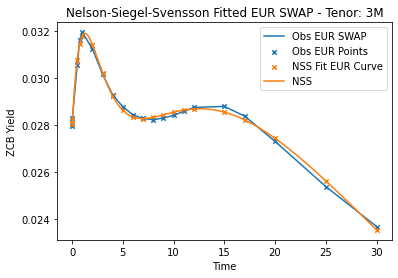
\includegraphics[width = 0.48\textwidth]{Plots/3M-EURIBOr_fit.png}}
\subfloat[6M EURIBOR]{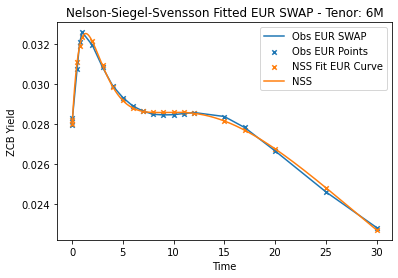
\includegraphics[width = 0.48\textwidth]{Plots/6M-EURIBOr_fit.png}}\\
\caption{Fitting of Swap curves to the NSS-model}
\label{fig:NSSfit}
\end{figure}
As seen in Figure~\ref{fig:NSSfit}
the two Swap Curves is fitted alright by the NSS model,
however we note that these rates
indicate that the initial forward rates
will decay rapidly, when
we go beyond the 15Y point as seen in Figure~\ref{fig:NSSfwdLib}.

\begin{figure}[H]
\subfloat[3M EURIBOR]{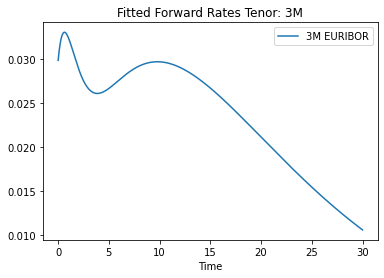
\includegraphics[width = 0.48\textwidth]{Plots/3M-EURIBOr_Fwd_Rates.png}}
\subfloat[6M EURIBOR]{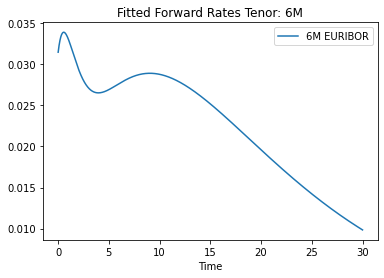
\includegraphics[width = 0.48\textwidth]{Plots/6M-EURIBOr_Fwd_Rates.png}}\\
\caption{Initial Forward Rate curve, $L_k^{x}(0)$,
for $x = \left\{ \text{3M}, \text{6M} \right\} $}
\label{fig:NSSfwdLib}
\end{figure}
% subsection fitting_initial_euribor_curve_ (end)

% subsection determining_ (end)

% subsubsection subsubsection_name (end)

%%%%% New Section %%%%%%%%
\section{Analysing the affect of xIBOR to OIS}
When comparing the Spread model in section \ref{sec:the_setup}
with different dependence structures with
the OIS model in section \ref{sec:the_setup}
we want to consider different aspects namely:
\begin{itemize}
     \item The initial price of a portfolio under
     the different parameterization of the spread model
     compared to the single curve RFR-model of (\ref{eq:vasicekdynamics}).
     \item The implied volatility for different Maturities
     and more importantly what level of short rate
     volatility is needed to generate the implied volatility levels.
 \end{itemize}
What we thus consider is the relative
volatility change on the underlying short rate
one could assume will appear when modelling and fitting
ATM-volatilities. The hypothesis
is that Spread models with relative
large depence structure(ie. correlation, $\rho^x$, and
spread vol, $v^x$) will have a relative large impact on the
the calibrated short rate vol, $\sigma$, whenever they are fitted
to ATM volatility for the deterministic case of the spread model,
hence when $\alpha^x = \beta ^x = 0$. \newline

Firstly we note that the strike of an ATM Cap is
just the initial swap rate with the floating
and fixed leg paying at the same times.
So for an OIS-Cap we have:
\begin{equation}
    \bar K = S^{OIS}_{a , b}(0) = \frac{\sum_{k=a+1}^b\tau_k P_D(0,T_k)F_k(0)}
    {\sum_{k=a+1}^b\tau_k P_D(0,T_k)} = \frac{P_D(0,T_a) - P_D(0,T_b)}{\sum_{k=a+1}^b\tau_k P_D(0,T_k)}
\end{equation}
and for the EURIBOR Cap it is given by:
\begin{equation}
    \bar K = S^{Spr}_{a,b}(0) = \frac{\sum_{k=a+1}^b\tau_k P_D(0,T_k)L_k(0)}
    {\sum_{k=a+1}^b\tau_k P_D(0,T_k)}
\end{equation}
The initial data we use for our
short-rate model in (\ref{eq:vasicekdynamics}) is:
\begin{equation}
    \notag \kappa = 0.06,~   \theta = 0.253 ,~ \sigma = 0.011 ,~ r(0) = 0.0279
\end{equation}
and for the Stochastic basis in (\ref{eq:BasisSpreadDef}) we set $\eta = 0.5$.
We consider two tenor structures namely 3M and 6M and for
these we consider the dependence structures:
\begin{equation}\notag
    \begin{aligned}
        \rho^{3M} = \left\{ 0 , - 0.60232 \right\}, ~v^{3M} = \left\{ 0.0 , 0.0218 , 0.04491 , 0.03316 \right\} \\
        \rho^{6M} = \left\{ 0 , - 0.62067 \right\}, ~v^{6M} = \left\{ 0.0 , 0.02448 , 0.03308 , 0.02868 \right\}
    \end{aligned}
\end{equation}
In Figure~\ref{fig:BlackImVol},
Figure~\ref{fig:BachImVol} and Table~\ref{tab:CalShortVol}
we see the volatility skews, smirks and a smile generated
by finding the implied volatility for the Black and Bachelier
model respectively. Starting at the deterministic basis $\alpha ^x = \beta^x =0$
and calibrating $ \sigma$ for our other models to hit the ATM volatility for
Caps of 10Y's payments starting after one quarter of year.
Just as in \cite{MercXieStochBasis2012} we see
that our deterministic basis makes the biggest skew and that
the parameterization closest to have a similar implied volatility structure
as our OIS model is the model with the largest dependence parameters.
However this shall not trick us - If we take a look at Table~\ref{tab:CalShortVol}
we observe that it is actually the model that differs the most
with our recalibrated short vol parameter, $\sigma$,
being around twice to four times as small.
This intuitively indicates that if the OIS model and for instance
the Spread model with $\alpha^{3M} = 0.0$ and $\beta^{3M} = 0.02245$
were to have the same short rate volatility, $\sigma$ the implied volatility,
would be on a way higher(if not ridiculous higher) level than our OIS model.
Another thing to note is that for the Black implied volatilities
it merely only skew and a single smirk that is observed,
where as the shapes gets a bit more funky/wild when considering the Bachelier implied volatilities.
This can also be due to the implied vol of the bachelier model is quoted in nominal(Basis points),
whereas Black volatilities are percentages.\newline

Now turning our attention to Table~\ref{tab:AtmCapPrice},
Table~\ref{tab:ITMCapPrice} and Table~\ref{tab:OTMCapPrice}.
Here $\sigma$ is not calibrated to match any implied volatilities.\footnote{One
could try to do so to see if that would have an interesting effect.}
We see that the prices actually follows quite nicely
as maturity increases(although one would wonder whether the prices are rather large - The
same could one think about the implied volatilities above).
None of the parameterizations that dramatically increase or decrease.
The dependence structures that has the highest prices
are also the ones who differed the most in the $\sigma$ calibration from above.
Although it is remarkable that
the prices for all spread models are so much higher than the OIS model, consequently
at least twice as large. This could be
due to the simplistic OIS model that is not initially fitted to data(and might have
a unrealistic forward curve) and is 'internally
priced', since $F_k(t)$ are generated from the discount factors.

\begin{figure}[H]
\subfloat[$x=$ 3M, $\rho = 0.0$]{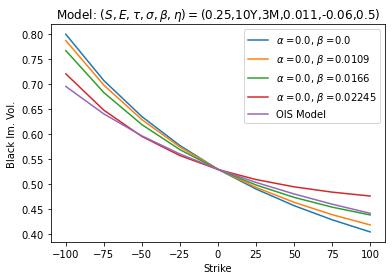
\includegraphics[width = 0.48\textwidth]{Plots/BlackImVol-rho-False-3M.png}}
\subfloat[$x=$ 3M, $\rho = -0.6023$]{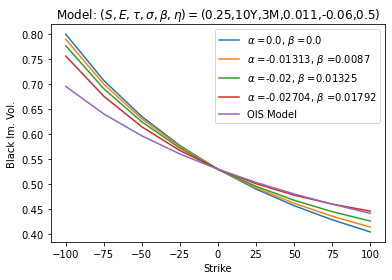
\includegraphics[width = 0.48\textwidth]{Plots/BlackImVol-rho-True-3M.png}}\\
\subfloat[$x=$ 6M, $\rho = 0.0$]{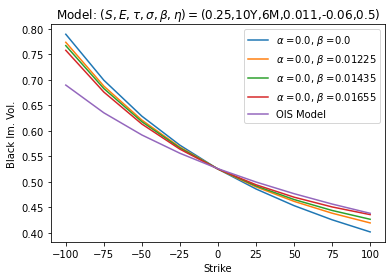
\includegraphics[width = 0.48\textwidth]{Plots/BlackImVol-rho-False-6M_1.png}}
\subfloat[$x=$ 6M, $\rho = -0.6210$]{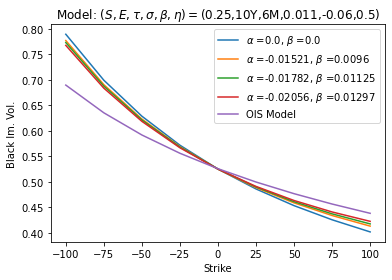
\includegraphics[width = 0.48\textwidth]{Plots/BlackImVol-rho-True-6M_1.png}}
\caption{Black Implied Volatilities}
\label{fig:BlackImVol}
\end{figure}
\begin{figure}[H]
\subfloat[$x=$ 3M, $\rho = 0.0$]{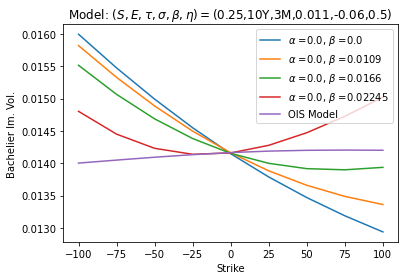
\includegraphics[width = 0.48\textwidth]{Plots/BachImVol-rho-False-3M.png}}
\subfloat[$x=$ 3M, $\rho = -0.6023$]{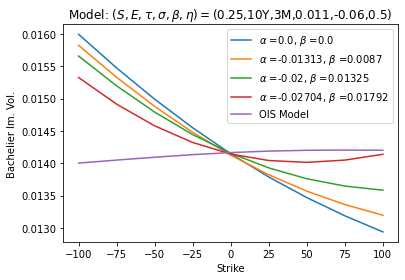
\includegraphics[width = 0.48\textwidth]{Plots/BachImVol-rho-True-3M.png}}\\
\subfloat[$x=$ 6M, $\rho = 0.0$]{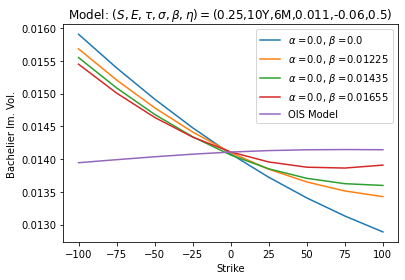
\includegraphics[width = 0.48\textwidth]{Plots/BachImVol-rho-False-6M_1.png}}
\subfloat[$x=$ 6M, $\rho = -0.6210$]{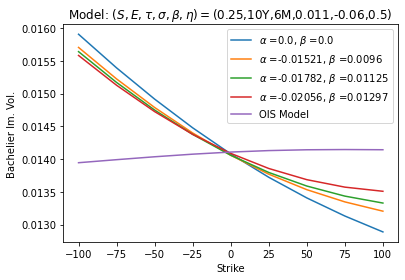
\includegraphics[width = 0.48\textwidth]{Plots/BachImVol-rho-True-6M_1.png}}
\caption{Bachelier Implied Volatilities}
\label{fig:BachImVol}
\end{figure}
\begin{table}[H]
    \centering
    \begin{tabular}{|c||c||c||c|c|} \hline
    Tenor               & $\alpha^x$          & $\beta^x$                     &  Bachelier    & Black \\ \hline \hline
    \multirow{8}{*}{3M} & \multirow{4}{*}{0.0}  & \multicolumn{1}{l||}{0.0} & \multicolumn{1}{l|}{0.011} & \multicolumn{1}{l|}{ 0.011} \\\cline{3-5}
                        &                          & \multicolumn{1}{l||}{0.00109} & \multicolumn{1}{l|}{0.0091437} & \multicolumn{1}{l|}{0.00912656} \\\cline{3-5}
                        &                          & \multicolumn{1}{l||}{0.0166} & \multicolumn{1}{l|}{0.0071435} & \multicolumn{1}{l|}{0.00713012} \\\cline{3-5}
                        &                          & \multicolumn{1}{l||}{0.02245} & \multicolumn{1}{l|}{0.0036610} & \multicolumn{1}{l|}{0.0036096} \\\cline{2-5}
                        & \multicolumn{1}{l||}{-0.01313} & \multicolumn{1}{l||}{0.0087} & \multicolumn{1}{l|}{ 0.009900} & \multicolumn{1}{l|}{0.0099343} \\\cline{2-5}
                        & \multicolumn{1}{l||}{-0.02} & \multicolumn{1}{l||}{0.01325} & \multicolumn{1}{l|}{0.008724} & \multicolumn{1}{l|}{0.008715} \\\cline{2-5}
                        & \multicolumn{1}{l||}{-0.02704} & \multicolumn{1}{l||}{0.01792} & \multicolumn{1}{l|}{0.0069249} & \multicolumn{1}{l|}{0.0069454} \\\cline{2-5}
                        &  \multicolumn{2}{|c||}{OIS}                          &  \multicolumn{1}{l|}{0.0166375} & \multicolumn{1}{l|}{0.0146781} \\ \hline \hline
    \multirow{8}{*}{6M}& \multirow{4}{*}{0.0} & \multicolumn{1}{l||}{0.0} & \multicolumn{1}{l|}{0.011} & \multicolumn{1}{l|}{0.011} \\\cline{3-5}
                        &                          & \multicolumn{1}{l||}{0.01225} & \multicolumn{1}{l|}{0.008731} & \multicolumn{1}{l|}{0.008705} \\\cline{3-5}
                        &                          & \multicolumn{1}{l||}{0.01435} & \multicolumn{1}{l|}{0.007967} & \multicolumn{1}{l|}{0.007998} \\\cline{3-5}
                        &                          & \multicolumn{1}{l||}{0.01655} & \multicolumn{1}{l|}{0.007170} & \multicolumn{1}{l|}{0.007129} \\\cline{2-5}
                        & \multicolumn{1}{l||}{-0.01521} & \multicolumn{1}{l||}{0.0096} & \multicolumn{1}{l|}{0.00969375} & \multicolumn{1}{l|}{0.009719531} \\\cline{2-5}
                        & \multicolumn{1}{l||}{-0.01782} & \multicolumn{1}{l||}{0.01125} & \multicolumn{1}{l|}{0.00930189} & \multicolumn{1}{l|}{0.009301895} \\\cline{2-5}
                        & \multicolumn{1}{l||}{-0.02056} & \multicolumn{1}{l||}{0.01297} & \multicolumn{1}{l|}{0.0088061} & \multicolumn{1}{l|}{0.008793} \\\hline
                        &  \multicolumn{2}{|c||}{OIS}                          &  \multicolumn{1}{l|}{0.01656875} & \multicolumn{1}{l|}{0.0147640} \\ \hline
     \end{tabular}
    \caption{Calibrated short rate volatilities $\sigma$ to fit ATM Volatility for the Deterministic basis.}
    \label{tab:CalShortVol}
\end{table}
\begin{table}[H]
    \centering
    \begin{tabular}{|c||c||c||c|c|c|c|c|} \hline
    Tenor               & $\alpha^x$          & $\beta^x$                               &  5Y                      & 10Y                      & 15Y                     & 20Y                   & 25Y   \\ \hline \hline
    \multirow{8}{*}{3M} & \multirow{4}{*}{0.0}  & \multicolumn{1}{l||}{0.0}             & \multicolumn{1}{l|}{3.88\%}    & \multicolumn{1}{l|}{10.3\%}      & \multicolumn{1}{l|}{17.66\%} & \multicolumn{1}{l|}{25.3\%} & \multicolumn{1}{l|}{32.98\%}\\\cline{3-8}
                        &                          & \multicolumn{1}{l||}{0.00109}      & \multicolumn{1}{l|}{4.27\%} & \multicolumn{1}{l|}{11.31\%}     & \multicolumn{1}{l|}{19.34\%} & \multicolumn{1}{l|}{27.68\%} & \multicolumn{1}{l|}{36.09\%}\\\cline{3-8}
                        &                          & \multicolumn{1}{l||}{0.0166}       & \multicolumn{1}{l|}{4.66\%} & \multicolumn{1}{l|}{12.23\%}      & \multicolumn{1}{l|}{20.81\%} & \multicolumn{1}{l|}{29.69\%} & \multicolumn{1}{l|}{38.41\%}\\\cline{3-8}
                        &                          & \multicolumn{1}{l||}{0.02245}      & \multicolumn{1}{l|}{5.14\%} & \multicolumn{1}{l|}{13.37\%}      & \multicolumn{1}{l|}{22.61\%} & \multicolumn{1}{l|}{32.14\%} & \multicolumn{1}{l|}{41.68\%}\\\cline{2-8}
                        & \multicolumn{1}{l||}{-0.01313} & \multicolumn{1}{l||}{0.0087}  & \multicolumn{1}{l|}{4.1\%}    & \multicolumn{1}{l|}{10.88\%} & \multicolumn{1}{l|}{18.64\%} & \multicolumn{1}{l|}{26.7\%}& \multicolumn{1}{l|}{34.83\%} \\\cline{2-8}
                        & \multicolumn{1}{l||}{-0.02} & \multicolumn{1}{l||}{0.01325}    & \multicolumn{1}{l|}{4.35\%}     & \multicolumn{1}{l|}{11.48\%} & \multicolumn{1}{l|}{19.58\%} & \multicolumn{1}{l|}{27.99\%}& \multicolumn{1}{l|}{36.45\%} \\\cline{2-8}
                        & \multicolumn{1}{l||}{-0.02704} & \multicolumn{1}{l||}{0.01792}  & \multicolumn{1}{l|}{4.67\%}     & \multicolumn{1}{l|}{12.23\%} & \multicolumn{1}{l|}{20.77\%} & \multicolumn{1}{l|}{29.59\%}& \multicolumn{1}{l|}{38.46\%} \\\cline{2-8}
                        &  \multicolumn{2}{|c||}{OIS}                                   &  \multicolumn{1}{l|}{2.28\%} & \multicolumn{1}{l|}{5.41\%}      & \multicolumn{1}{l|}{8.3\%} & \multicolumn{1}{l|}{11.44\%} & \multicolumn{1}{l|}{14.91\%}\\ \hline \hline
    \multirow{8}{*}{6M}& \multirow{4}{*}{0.0} & \multicolumn{1}{l||}{0.0}               & \multicolumn{1}{l|}{3.74\%}    & \multicolumn{1}{l|}{10.06\%}   & \multicolumn{1}{l|}{17.32\%} & \multicolumn{1}{l|}{24.89\%} & \multicolumn{1}{l|}{32.53\%}\\\cline{3-8}
                        &                          & \multicolumn{1}{l||}{0.01225}      & \multicolumn{1}{l|}{4.2\%} & \multicolumn{1}{l|}{11.25\%}      & \multicolumn{1}{l|}{19.31\%} & \multicolumn{1}{l|}{27.71\%} & \multicolumn{1}{l|}{36.18\%}\\\cline{3-8}
                        &                          & \multicolumn{1}{l||}{0.01435}      & \multicolumn{1}{l|}{4.33\%} &  \multicolumn{1}{l|}{11.58\%}     & \multicolumn{1}{l|}{19.84\%} & \multicolumn{1}{l|}{28.44\%} & \multicolumn{1}{l|}{37.1\%}\\\cline{3-8}
                        &                          & \multicolumn{1}{l||}{0.01655}      & \multicolumn{1}{l|}{4.49\%} &   \multicolumn{1}{l|}{11.96\%}    & \multicolumn{1}{l|}{20.44\%} & \multicolumn{1}{l|}{29.25\%} & \multicolumn{1}{l|}{38.12\%}\\\cline{2-8}
                        & \multicolumn{1}{l||}{-0.01521} & \multicolumn{1}{l||}{0.0096} & \multicolumn{1}{l|}{3.99\%} & \multicolumn{1}{l|}{10.73\%}      & \multicolumn{1}{l|}{18.45\%} & \multicolumn{1}{l|}{26.51\%} & \multicolumn{1}{l|}{34.65\%}\\\cline{2-8}
                        & \multicolumn{1}{l||}{-0.01782} & \multicolumn{1}{l||}{0.01125} & \multicolumn{1}{l|}{4.08\%} & \multicolumn{1}{l|}{10.94\%}     & \multicolumn{1}{l|}{18.78\%} & \multicolumn{1}{l|}{26.97\%} & \multicolumn{1}{l|}{35.22\%}\\\cline{2-8}
                        & \multicolumn{1}{l||}{-0.02056} & \multicolumn{1}{l||}{0.01297} & \multicolumn{1}{l|}{4.18\%} & \multicolumn{1}{l|}{11.17\%}     & \multicolumn{1}{l|}{19.16\%} & \multicolumn{1}{l|}{27.48\%} & \multicolumn{1}{l|}{35.86\%}\\\cline{2-8}
                        &  \multicolumn{2}{|c||}{OIS}                                   &  \multicolumn{1}{l|}{2.14\%} & \multicolumn{1}{l|}{5.34\%}      & \multicolumn{1}{l|}{8.43\%} & \multicolumn{1}{l|}{11.78\%} & \multicolumn{1}{l|}{15.44\%}\\ \hline
     \end{tabular}
    \caption{Price in \% of notional for ATM Cap prices for our considered tenor structures
    and dependence structures.}
    \label{tab:AtmCapPrice}
\end{table}
\begin{table}[H]
    \centering
    \begin{tabular}{|c||c||c||c|c|c|c|c|} \hline
    Tenor               & $\alpha^x$          & $\beta^x$                               &  5Y                      & 10Y                      & 15Y                     & 20Y                   & 25Y   \\ \hline \hline
    \multirow{8}{*}{3M} & \multirow{4}{*}{0.0}  & \multicolumn{1}{l||}{0.0}             & \multicolumn{1}{l|}{5.45\%}    & \multicolumn{1}{l|}{13.29\%}      & \multicolumn{1}{l|}{21.98\%} & \multicolumn{1}{l|}{30.9\%} & \multicolumn{1}{l|}{39.80\%}\\\cline{3-8}
                        &                          & \multicolumn{1}{l||}{0.00109}      & \multicolumn{1}{l|}{5.77\%} & \multicolumn{1}{l|}{14.13\%}     & \multicolumn{1}{l|}{23.38\%} & \multicolumn{1}{l|}{32.88\%} & \multicolumn{1}{l|}{42.38\%}\\\cline{3-8}
                        &                          & \multicolumn{1}{l||}{0.0166}       & \multicolumn{1}{l|}{6.09\%} & \multicolumn{1}{l|}{14.90\%}      & \multicolumn{1}{l|}{24.62\%} & \multicolumn{1}{l|}{34.58\%} & \multicolumn{1}{l|}{44.52\%}\\\cline{3-8}
                        &                          & \multicolumn{1}{l||}{0.02245}      & \multicolumn{1}{l|}{5.50\%} & \multicolumn{1}{l|}{15.88\%}      & \multicolumn{1}{l|}{26.17\%} & \multicolumn{1}{l|}{36.69\%} & \multicolumn{1}{l|}{47.17\%}\\\cline{2-8}
                        & \multicolumn{1}{l||}{-0.01313} & \multicolumn{1}{l||}{0.0087}  & \multicolumn{1}{l|}{5.62\%}    & \multicolumn{1}{l|}{13.75\%} & \multicolumn{1}{l|}{22.75\%} & \multicolumn{1}{l|}{32.01\%}& \multicolumn{1}{l|}{41.26\%} \\\cline{2-8}
                        & \multicolumn{1}{l||}{-0.02} & \multicolumn{1}{l||}{0.01325}    & \multicolumn{1}{l|}{5.82\%}     & \multicolumn{1}{l|}{14.23\%} & \multicolumn{1}{l|}{23.52\%} & \multicolumn{1}{l|}{33.06\%}& \multicolumn{1}{l|}{42.58\%} \\\cline{2-8}
                        & \multicolumn{1}{l||}{-0.02704} & \multicolumn{1}{l||}{0.01792}  & \multicolumn{1}{l|}{6.09\%}     & \multicolumn{1}{l|}{14.86\%} & \multicolumn{1}{l|}{24.51\%} & \multicolumn{1}{l|}{34.39\%}& \multicolumn{1}{l|}{44.25\%} \\\cline{2-8}
                        &  \multicolumn{2}{|c||}{OIS}                                   &  \multicolumn{1}{l|}{3.54\%} & \multicolumn{1}{l|}{7.62\%}      & \multicolumn{1}{l|}{11.30\%} & \multicolumn{1}{l|}{15.25\%} & \multicolumn{1}{l|}{19.55\%}\\ \hline \hline
    \multirow{8}{*}{6M}& \multirow{4}{*}{0.0} & \multicolumn{1}{l||}{0.0}               & \multicolumn{1}{l|}{5.31\%}    & \multicolumn{1}{l|}{13.05\%}   & \multicolumn{1}{l|}{21.64\%} & \multicolumn{1}{l|}{30.49\%} & \multicolumn{1}{l|}{39.33\%}\\\cline{3-8}
                        &                          & \multicolumn{1}{l||}{0.01225}      & \multicolumn{1}{l|}{5.69\%} & \multicolumn{1}{l|}{14.04\%}      & \multicolumn{1}{l|}{23.30\%} & \multicolumn{1}{l|}{32.84\%} & \multicolumn{1}{l|}{42.38\%}\\\cline{3-8}
                        &                          & \multicolumn{1}{l||}{0.01435}      & \multicolumn{1}{l|}{5.8\%} &  \multicolumn{1}{l|}{14.32\%}     & \multicolumn{1}{l|}{23.75\%} & \multicolumn{1}{l|}{33.45\%} & \multicolumn{1}{l|}{43.15\%}\\\cline{3-8}
                        &                          & \multicolumn{1}{l||}{0.01655}      & \multicolumn{1}{l|}{5.93\%} &   \multicolumn{1}{l|}{14.64\%}    & \multicolumn{1}{l|}{24.26\%} & \multicolumn{1}{l|}{34.15\%} & \multicolumn{1}{l|}{38.12\%}\\\cline{2-8}
                        & \multicolumn{1}{l||}{-0.01521} & \multicolumn{1}{l||}{0.0096} & \multicolumn{1}{l|}{5.51\%} & \multicolumn{1}{l|}{13.58\%}      & \multicolumn{1}{l|}{22.54\%} & \multicolumn{1}{l|}{31.78\%} & \multicolumn{1}{l|}{41.02\%}\\\cline{2-8}
                        & \multicolumn{1}{l||}{-0.01782} & \multicolumn{1}{l||}{0.01125} & \multicolumn{1}{l|}{5.58\%} & \multicolumn{1}{l|}{13.75\%}     & \multicolumn{1}{l|}{22.81\%} & \multicolumn{1}{l|}{32.14\%} & \multicolumn{1}{l|}{41.48\%}\\\cline{2-8}
                        & \multicolumn{1}{l||}{-0.02056} & \multicolumn{1}{l||}{0.01297} & \multicolumn{1}{l|}{5.66\%} & \multicolumn{1}{l|}{13.94\%}     & \multicolumn{1}{l|}{23.12\%} & \multicolumn{1}{l|}{32.56\%} & \multicolumn{1}{l|}{42.00\%}\\\cline{2-8}
                        &  \multicolumn{2}{|c||}{OIS}                                   &  \multicolumn{1}{l|}{3.34\%} & \multicolumn{1}{l|}{7.54\%}      & \multicolumn{1}{l|}{11.46\%} & \multicolumn{1}{l|}{15.67\%} & \multicolumn{1}{l|}{20.19\%}\\ \hline
     \end{tabular}
    \caption{Price in \% of notional for ITM (with 50 BP) Cap prices for our considered tenor structures
    and dependence structures.}
    \label{tab:ITMCapPrice}
\end{table}

\begin{table}[H]
    \centering
    \begin{tabular}{|c||c||c||c|c|c|c|c|} \hline
    Tenor               & $\alpha^x$          & $\beta^x$                               &  5Y                      & 10Y                      & 15Y                     & 20Y                   & 25Y   \\ \hline \hline
    \multirow{8}{*}{3M} & \multirow{4}{*}{0.0}  & \multicolumn{1}{l||}{0.0}             & \multicolumn{1}{l|}{2.61\%}    & \multicolumn{1}{l|}{7.77\%}      & \multicolumn{1}{l|}{13.91\%} & \multicolumn{1}{l|}{20.35\%} & \multicolumn{1}{l|}{26.87\%}\\\cline{3-8}
                        &                          & \multicolumn{1}{l||}{0.00109}      & \multicolumn{1}{l|}{3.05\%} & \multicolumn{1}{l|}{8.92\%}     & \multicolumn{1}{l|}{15.85\%} & \multicolumn{1}{l|}{23.12\%} & \multicolumn{1}{l|}{30.49\%}\\\cline{3-8}
                        &                          & \multicolumn{1}{l||}{0.0166}       & \multicolumn{1}{l|}{3.50\%} & \multicolumn{1}{l|}{9.97\%}      & \multicolumn{1}{l|}{17.53\%} & \multicolumn{1}{l|}{25.42\%} & \multicolumn{1}{l|}{33.40\%}\\\cline{3-8}
                        &                          & \multicolumn{1}{l||}{0.02245}      & \multicolumn{1}{l|}{4.03\%} & \multicolumn{1}{l|}{11.24\%}      & \multicolumn{1}{l|}{19.55\%} & \multicolumn{1}{l|}{28.18\%} & \multicolumn{1}{l|}{36.87\%}\\\cline{2-8}
                        & \multicolumn{1}{l||}{-0.01313} & \multicolumn{1}{l||}{0.0087}  & \multicolumn{1}{l|}{2.87\%}    & \multicolumn{1}{l|}{8.45\%} & \multicolumn{1}{l|}{15.08\%} & \multicolumn{1}{l|}{22.04\%}& \multicolumn{1}{l|}{29.11\%} \\\cline{2-8}
                        & \multicolumn{1}{l||}{-0.02} & \multicolumn{1}{l||}{0.01325}    & \multicolumn{1}{l|}{3.16\%}     & \multicolumn{1}{l|}{9.15\%} & \multicolumn{1}{l|}{16.19\%} & \multicolumn{1}{l|}{23.57\%}& \multicolumn{1}{l|}{31.03\%} \\\cline{2-8}
                        & \multicolumn{1}{l||}{-0.02704} & \multicolumn{1}{l||}{0.01792}  & \multicolumn{1}{l|}{3.53\%}     & \multicolumn{1}{l|}{10.02\%} & \multicolumn{1}{l|}{17.56\%} & \multicolumn{1}{l|}{25.43\%}& \multicolumn{1}{l|}{33.38\%} \\\cline{2-8}
                        &  \multicolumn{2}{|c||}{OIS}                                   &  \multicolumn{1}{l|}{1.41\%} & \multicolumn{1}{l|}{3.75\%}      & \multicolumn{1}{l|}{5.98\%} & \multicolumn{1}{l|}{8.42\%} & \multicolumn{1}{l|}{11.14\%}\\ \hline \hline
    \multirow{8}{*}{6M}& \multirow{4}{*}{0.0} & \multicolumn{1}{l||}{0.0}               & \multicolumn{1}{l|}{2.48\%}    & \multicolumn{1}{l|}{7.53\%}   & \multicolumn{1}{l|}{13.57\%} & \multicolumn{1}{l|}{19.94\%} & \multicolumn{1}{l|}{26.42\%}\\\cline{3-8}
                        &                          & \multicolumn{1}{l||}{0.01225}      & \multicolumn{1}{l|}{3.0\%} & \multicolumn{1}{l|}{8.9\%}      & \multicolumn{1}{l|}{15.87\%} & \multicolumn{1}{l|}{23.21\%} & \multicolumn{1}{l|}{30.68\%}\\\cline{3-8}
                        &                          & \multicolumn{1}{l||}{0.01435}      & \multicolumn{1}{l|}{3.15\%} &  \multicolumn{1}{l|}{9.27\%}     & \multicolumn{1}{l|}{16.47\%} & \multicolumn{1}{l|}{24.05\%} & \multicolumn{1}{l|}{31.73\%}\\\cline{3-8}
                        &                          & \multicolumn{1}{l||}{0.01655}      & \multicolumn{1}{l|}{3.33\%} &   \multicolumn{1}{l|}{9.7\%}    & \multicolumn{1}{l|}{17.15\%} & \multicolumn{1}{l|}{24.98\%} & \multicolumn{1}{l|}{32.9\%}\\\cline{2-8}
                        & \multicolumn{1}{l||}{-0.01521} & \multicolumn{1}{l||}{0.0096} & \multicolumn{1}{l|}{2.77\%} & \multicolumn{1}{l|}{8.32 \%}      & \multicolumn{1}{l|}{14.92\%} & \multicolumn{1}{l|}{21.89\%} & \multicolumn{1}{l|}{28.99\%}\\\cline{2-8}
                        & \multicolumn{1}{l||}{-0.01782} & \multicolumn{1}{l||}{0.01125} & \multicolumn{1}{l|}{2.87\%} & \multicolumn{1}{l|}{8.57\%}     & \multicolumn{1}{l|}{15.31\%} & \multicolumn{1}{l|}{22.43\%} & \multicolumn{1}{l|}{29.67\%}\\\cline{2-8}
                        & \multicolumn{1}{l||}{-0.02056} & \multicolumn{1}{l||}{0.01297} & \multicolumn{1}{l|}{2.99\%} & \multicolumn{1}{l|}{8.84\%}     & \multicolumn{1}{l|}{15.75\%} & \multicolumn{1}{l|}{23.03\%} & \multicolumn{1}{l|}{30.43\%}\\\cline{2-8}
                        &  \multicolumn{2}{|c||}{OIS}                                   &  \multicolumn{1}{l|}{1.32 \%} & \multicolumn{1}{l|}{3.7\%}      & \multicolumn{1}{l|}{6.08\%} & \multicolumn{1}{l|}{8.69\%} & \multicolumn{1}{l|}{11.56\%}\\ \hline
     \end{tabular}
    \caption{Price in \% of notional for OTM (with 50 BP) Cap prices for our considered tenor structures
    and dependence structures.}
    \label{tab:OTMCapPrice}
\end{table}
\section{Conclusion} % (fold)
\label{sec:conclusion_and_reflections}
Summing everything up
this project showcased
how a simple single curve model can be extenden
through a stochastic basis to price both derivatives
with both OIS and xIBOR rates as a reference rate.
In addition it showcased that it is almost possible to
infer same implied volatilities,
however only for Black implied vol.,
in the OIS and Spread model.
Nevertheless a further investigation
led an interesting finding that
the calibrated short rate volatilies to fit ATM implied volatilies
for the deterministic spread
model were quite low, which could indicate that the pricing
for some parameterization under a identical short rate vol, $\sigma$,
could be significantly larger. This
was confirmed when checking prices for ATM, ITM and OTM prices
for caps of different maturities, where the spread model
consistently had prices approximately twice as large as the OIS model.
This
could confirm that the era of OIS swaps
leads to lesser change in daily values on
derivatives contracts - Nevertheless this should be exmined further.

\textbf{}
% section conclusion_and_reflections (end)
% section the_setup (end)
% section convergence_of_early_exercise_boundary (end)
% section convergence_in_time_for_different_theta_schemes_ (end)
\newpage
%\addcontentsline{toc}{section}{References}
\printbibliography[heading=bibintoc]
\end{document}

